\documentclass[12pt]{amsart}
\usepackage[top = 1in, bottom = 1in, left =1in, right = 1in]{geometry}
\usepackage[utf8]{inputenc}
\usepackage{hyperref}
\usepackage{listings}
\usepackage{multimedia} % to embed movies in the PDF file
\usepackage{graphicx}
\usepackage{comment}
\usepackage[english]{babel}
\usepackage{amsfonts,amscd,amssymb,amsmath,mathrsfs}
\usepackage{wrapfig}
\usepackage{multirow}
\usepackage{verbatim,cite}
\usepackage{float}
\usepackage{cancel}
\usepackage{caption}
\usepackage{subcaption}
\usepackage{mathdots}
\usepackage{bbm}
\usepackage{tikz}
\usepackage{setspace}
\usepackage{empheq}
\usepackage{hyperref}

\usepackage{macros}

\newcommand{\iid}{\overset{\mathrm{iid}}{\sim}}


\title{Graphical Semi-Supervised Learning}

\author{Rohin Gilman \and Alex Johnson \and Kaitlynn Lilly}

\doublespacing
\begin{document}

\begin{abstract}
    We investigate graphical semi-supervised learning approaches and benchmark both Probit and regression models on various manifolds. We construct data on well-separated clusters in the plane, weakly connected clusters on a spiral manifold, and examine data from the MNIST data set. We find that these approaches are generally effective, but can be limited by the underlying data and choices made in model construction.
\end{abstract}

\maketitle

\section{Introduction} 
Graphical semi-supervised learning (GSSL) is a prominent field of research in machine learning as it serves as a powerful technique for dealing with classification problems in which only a small subset of the data is labeled. In kernel methods for GSSL, the unlabeled data is used to construct a similarity graph, where each node represents an instance and the edges indicate the similarity between them. Clustering this graph results in a complete labeling of the data set. As a result, GSSL using kernel methods is a promising approach for tackling problems in areas such as image recognition, natural language processing, and bioinformatics.

\section{Theoretical Background}

\subsection{Proximity Graphs}
Given a set of points $\{x_1, x_2, \dots, x_n\}$ in a metric space, we can construct a proximity graph $G = (V, W)$, where $V = \{v_1, v_2, \dots, v_n\}$ is a set of vertices representing the points, and $W$ is an adjacency matrix whose entries are
\[W_{ij} = \begin{cases}
  \eta(x_i,x_j) \quad&\text{if } d(x_i,x_j) < r, \\
  0 \quad&\text{otherwise},
\end{cases}\]
where $\eta\colon X\times X \to \R$ is a non-increasing function, and $r > 0$ is the radius within which vertices can be adjacent. These represent the weights of the edges between pairs of vertices.
\subsection{K-Nearest Neighbor Graphs}
K-Nearest Neighbor (K-NN) graphs are a class of graphs within which vertices are adjacent to a fixed number of other vertices. The K-NN graph $G_k = (V, W)$ is constructed as follows: for each vertex $v_i$, its $k$-nearest neighbors are found according to some distance metric, and edges of weight $\eta(x_1,x_2)$ are added between $v_i$ and each of its $k$-nearest neighbors. In other words, $v_i$ is adjacent to the $k$ vertices that are closest to it in the data set. The primary advantage of using K-NN graphs is that on average, vertices have relatively low degree, so the weight matrix $W$ is often sparse, increasing the performance of graphical methods.

\subsection{Graph Laplacian}
Given a graph $G = (V, W)$, we can define a graph Laplacian $L$ as a matrix that captures the pairwise relationships between data points on the graph. Specifically, we can construct the unnormalized graph Laplacian $L$ as follows:
$$ L = D - W, $$
where $D$ is the diagonal degree matrix defined by
\[D_{ii} = \sum_{j = 1}^n W_{ij}.\]
If $G$ has $M$ connected components, then $\mathrm{dim}(\mathrm{Null}(L))=M$. Thus, we only need to find the multiplicity of the zero-eigenvalue of $L$ to determine the number of clusters in the data.
\begin{comment}
In GSSL, we can use the Laplacian to propagate labels from a small set of labeled data points to the entire graph, by solving the following optimization problem:
$$ \min_f \sum_i L_{ii} (f_i - y_i)^2 + \lambda \sum_{i,j} W_{ij} (f_i - f_j)^2, $$
where $y_i$ is the label for the $i$-th labeled point, $f_i$ is the predicted label for the $i$-th point, and $\lambda$ is a regularization parameter that controls the smoothness of the solution. 
\end{comment}

\subsection{Matérn Family of Kernels}
We define the Matérn kernel as
\[
  K(x,y) = \kappa(\norm{x-y}), \kappa(t) = \frac{2^{1-\nu}}{\Gamma(\nu)}\paren{\sqrt{2\nu}\frac{t}{\gamma}}K_{\nu}\paren{\sqrt{2\nu}\frac{t}{\gamma}},
\]
where $\Gamma$ is the Gamma function, $K_{\nu}$ is the modified Bessel function of the second kind, $\nu$ is a smoothness index, and $\gamma$ is the length scale. It has been shown that Matérn kernels on Gaussian Processes satisfy the PDE operator
\[
  \paren{\frac{2\nu}{\gamma ^2} + \Delta}^{\frac{\nu}{2} + \frac{d}{4}},
\]
where $d$ is the dimension of $x$ and $y$, and $\Delta$ is the Laplacian operator. On finite graphs, after we redefine variables, the discrete Matérn kernel is then defined as
\[
  C = \paren{L + \tau^2 I}^{-\alpha},
\]
where $L$ is the graph Laplacian matrix, and $\tau$, $\alpha$ are refactored terms.

\subsection{The Probit Method}\label{Sec:Probit}
The probit method is a statistical technique used for modeling binary response variables. We assume
\[y_j = \mathrm{sign}(f(x_j) + \epsilon_j),\]
for some latent function $f$, where $\epsilon_j\iid \psi$, for some probability density $\psi$. Assume $\psi$ is symmetric, so that
\begin{align*}
	\mathbb{P}(y_j = +1 \mid f) &= \mathbb{P}(f(x_j) + \epsilon_j \geq 0) \\
	&= \mathbb{P}(\epsilon_j \geq - f(x_j)  ) \\
	&= \int_{-f(x_j)}^\infty \psi(t) \ddd t \\
	&= \int_{-\infty}^{f(x_j)} \psi(t) \ddd t \\
	&= \Psi(f(x_j)) \\
	&= \Psi(y_jf(x_j)),
\end{align*}
where $\Psi$ is the cumulative distribution function (CDF) of $\psi$. By the same calculation, we obtain $\mathbb{P}(y_j = -1 \mid f) = \Psi(y_jf(x_j))$. Thus, $\mathbb{P}(y_j \mid f) = \Psi(y_jf(x_j))$. Since the $\epsilon_j$ are independent and identically distributed, we can write
\[\mathbb{P}(y  \mid f) = \prod_{j = 1}^n \Psi(y_jf(x_j)).\]
For a function $f$, we want our loss function to be large when the signs of $f(x_j)$ and $y_j$  disagree, so we define our probit loss:
\[L(f) = -\log(\mathbb{P}(y\mid f)) = -\sum_{j = 1}^n \Psi(y_jf(x_j)).\]
Finally, we add a regularization term based on the RKHS norm to define our optimization problem for the probit method:
\[f^* = \argmin_{f \in \R^{m}} L(f) + \lambda f^{T}C^{-1}f.\]
Here, $C$ is as defined in Section 2.4. Since $C$ is defined from the graph Laplacian matrix, the optimization problem thus includes spectral information of $L$, hence embedding geometric cluster information in the assigning of labels when such a minimizing function is found.

\subsection{Regression}
Instead of using the probit model, we can instead use the simpler regression loss:
\[L(f) = \sum_{j = 1}^n \abs{f_j - y_j}^2.\]


\begin{comment}
In the kernel-based formulation of the probit method, the goal is to find the optimal values of the model coefficients, or dual variables, by maximizing the likelihood function. The likelihood function is defined as the product of the conditional probabilities of the response variable given the explanatory variables, which are modeled as a probit link function of a linear combination of kernel functions evaluated at the explanatory variables:
$$\mathbb{P}_r(y_i = 1 | \mathbf{x}_i) = \Phi(\mathbf{w}^\top \boldsymbol{\phi}(\mathbf{x}_i)),$$
where $y_i$ is the response variable for the $i$-th observation, $\mathbf{x}_i$ is the vector of explanatory variables, $\boldsymbol{\phi}(\cdot)$ is a nonlinear mapping of the input space to a high-dimensional feature space, $\mathbf{w}$ is a vector of model coefficients, and $\Phi(\cdot)$ is the cumulative distribution function of the standard normal distribution. The model coefficients are then estimated by solving an optimization problem of the form:
$$\min_{\mathbf{w}} \left[- \sum_{i=1}^n y_i \log \Phi(\mathbf{w}^\top \boldsymbol{\phi}(\mathbf{x}_i)) + (1 - y_i) \log (1 - \Phi(\mathbf{w}^\top \boldsymbol{\phi}(\mathbf{x}_i))) + \frac{\lambda}{2} \Vert \mathbf{w} \Vert^2\right],$$
where the first two terms correspond to the negative log-likelihood function, the third term is a regularization term that controls the complexity of the model, and $\lambda$ is the regularization parameter. This optimization problem can be solved using kernel ridge regression, which involves minimizing a regularized empirical risk function of the form:
$$\min_{\boldsymbol{\alpha}} \frac{1}{n} \sum_{i=1}^n \ell(y_i, f(\mathbf{x}_i)) + \frac{\lambda}{2} \boldsymbol{\alpha}^\top \mathbf{K} \boldsymbol{\alpha},$$
where $\boldsymbol{\alpha}$ are the dual variables, $f(\mathbf{x}_i) = \sum_{j=1}^n \alpha_j K(\mathbf{x}_i, \mathbf{x}_j)$ is the predicted probability for the $i$-th observation, $\ell(y_i, f(\mathbf{x}_i))$ is the loss function that measures the discrepancy between the observed response $y_i$ and the predicted probability $f(\mathbf{x}_i)$, $\lambda$ is the regularization parameter that controls the trade-off between fitting the data and the complexity of the model, and $\mathbf{K}$ is the kernel matrix whose entries are given by $K(\mathbf{x}_i, \mathbf{x}_j) = \boldsymbol{\phi}(\mathbf{x}_i)^\top \boldsymbol{\phi}(\mathbf{x}_j)$. 

\subsubsection{Spectral Clustering}
Spectral clustering is a clustering technique that uses the eigenvectors of a matrix derived from the data to cluster the data points. One common approach is to use the Laplacian matrix of the graph defined by the data points. Once we have the Laplacian matrix, we can compute its eigenvectors and eigenvalues. The eigenvectors corresponding to the smallest eigenvalues (excluding the first eigenvector, which is constant) are used as the embedding of the data points. The embedding maps the data points to a low-dimensional space, where the pairwise distances reflect the underlying structure of the data. Finally, we can use a clustering algorithm (e.g., k-means) to cluster the data points in the embedding space. The number of clusters can be determined using the number of zero eigenvalues of the graph Laplacian.

\end{comment}

\section{Methods}

\subsection{General Procedure}
\begin{enumerate}
    \item Data is obtained on a given manifold. True labels for the data are either extracted or assigned and are ultimately used to compute the accuracy of our approach.
    \item A graph is constructed from the unlabelled data, and is used to infer structure on the data. 
    \item The minimal latent function is determined by solving an optimization problem over the sum of a loss function using only the known labels and regularization term.
    \item The minimal latent function is used to predict the labels on all unlabelled vertices.
    \item The accuracy of the predicted labels using the true labels is computed.
\end{enumerate}

\subsection{Subproblems}

We now perform our general GSSL procedure on three different subproblems: three well separated clusters on the $\mathbb{R}^2$ manifold, three clusters on the swiss roll manifold, and the clusters generated using two digits from the MNIST data set. For each subproblem, we perform GSSL on a disconnected and weakly connected graph, except for MNIST, on which we only use a weakly connected graph. We compute our minimal latent function using probit and regression loss.

\section{Results}

\subsection{Clusters on $\mathbb{R}^2$}\label{Sec:3Clus}

We begin by generating the points to form well-separated clusters in $\mathbb{R}^2$. These clusters are formed by specifying the mean and a covariance matrix and the points are distributed normally. We demonstrate our results by choosing 3 clusters centered around $(0,0)$, $(1,0)$, and $(1,1)$, with 100 points in each cluster. One point in each cluster is then assigned its true label. Only these three assigned points will be used in our GSSL loss function. A plot of the clusters formed using this process is shown in Figure \ref{Fig:Dis3ClusOg}.

\begin{figure}
    \centering
    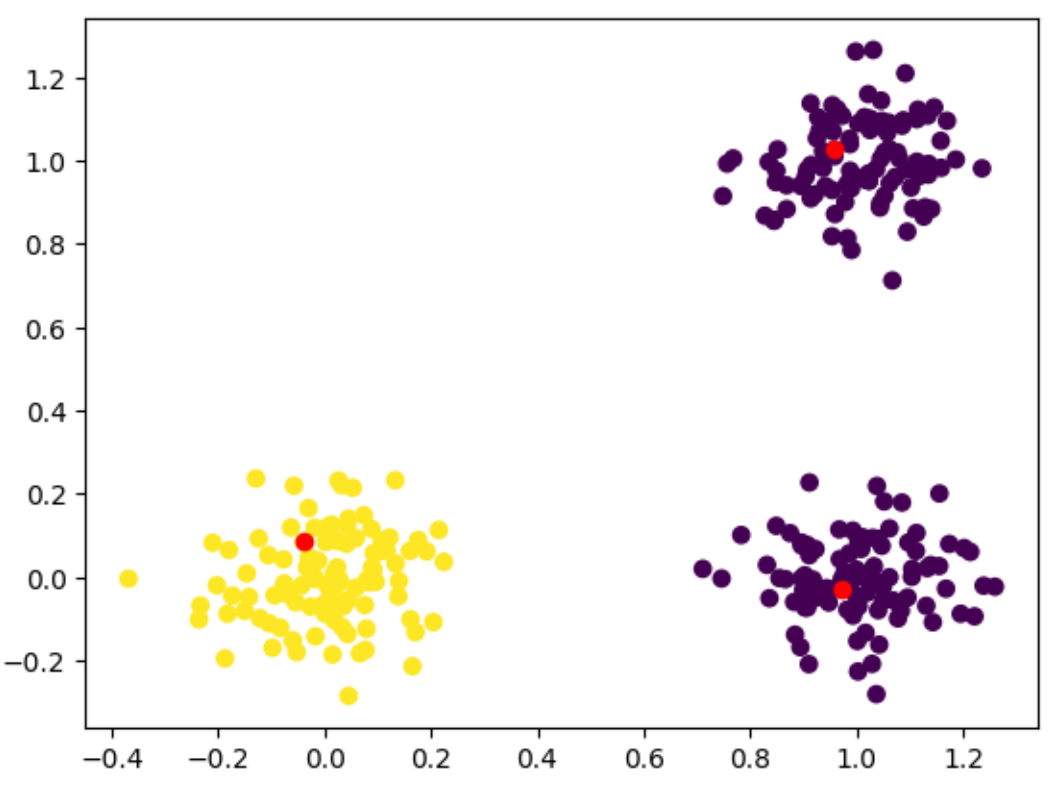
\includegraphics[width=0.5\textwidth]{Figures/Dis3ClusOG.png}
    \caption{
        Plot of the 3 well-separated clusters; the yellow points represent a label of $+1$, while purple points represent a label of $-1$. The red points indicate the points for which the label is known.}
	\label{Fig:Dis3ClusOg}
\end{figure}

We next use the data to construct a graph on the points. There are several choices to be made here, including the choice of weight function (and its parameters) and the type of graph. In this case, we explore two types of graphs: K-NN with uniform weights and proximity with Gaussian weights. We begin by examining the K-NN approach. This allows us to create a disconnected graph with 3 connected clusters. Such a graph constructed using this approach is shown in Figure \ref{Fig:Dis3ClusKNN}.

\begin{figure}
    \centering
    \begin{subfigure}[b]{0.475\textwidth}
      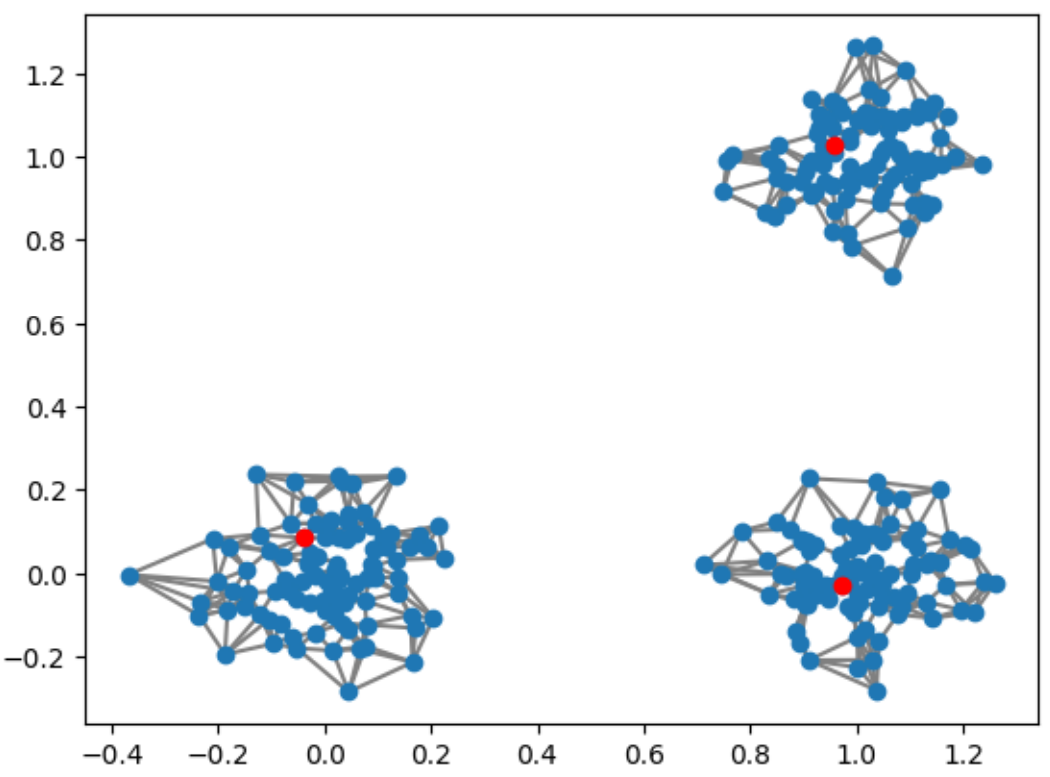
\includegraphics[width=\textwidth]{Figures/Dis3ClusKNN.png}
      \caption{K-NN Approach}
      \label{Fig:Dis3ClusKNN}
    \end{subfigure}
    \begin{subfigure}[b]{0.475\textwidth}
      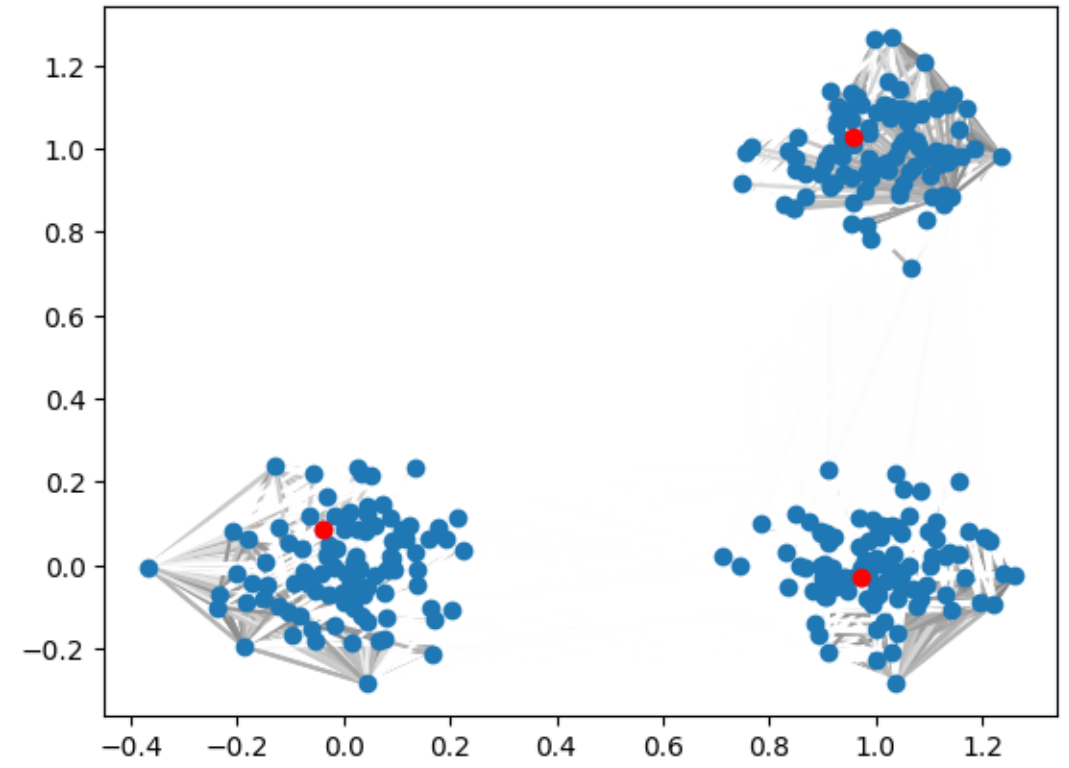
\includegraphics[width=\textwidth]{Figures/Dis3ClusProx.png}
      \caption{Proximity Approach}
      \label{Fig:Dis3ClusProx}
    \end{subfigure}
    \caption{
        Plot of the graphs constructed on the unlabelled data from Figure \ref{Fig:Dis3ClusOg}. Blue points indicate an unknown label, while red labels indicate known labels. The darker the shade of the edge, the higher its weight is.
    }
\end{figure}

We then perform our GSSL algorithm with both the Probit loss function and the regression loss function. Since the clusters in this case are completely disconnected, it was not necessary to tune any parameters in order to achieve an accuracy of 100\% using both loss functions. For each of these loss functions, we choose the following parameters: $\tau=1$, $\alpha=2$, and $\lambda=\frac{\tau^{2\alpha}}{2}$. Plots of the predicted labels using both the probit and regression loss functions are shown in Figure \ref{Fig:Dis3ClusKNNRes}.

    \begin{figure}[ht] 
  \begin{subfigure}{0.475\linewidth}
    \centering
    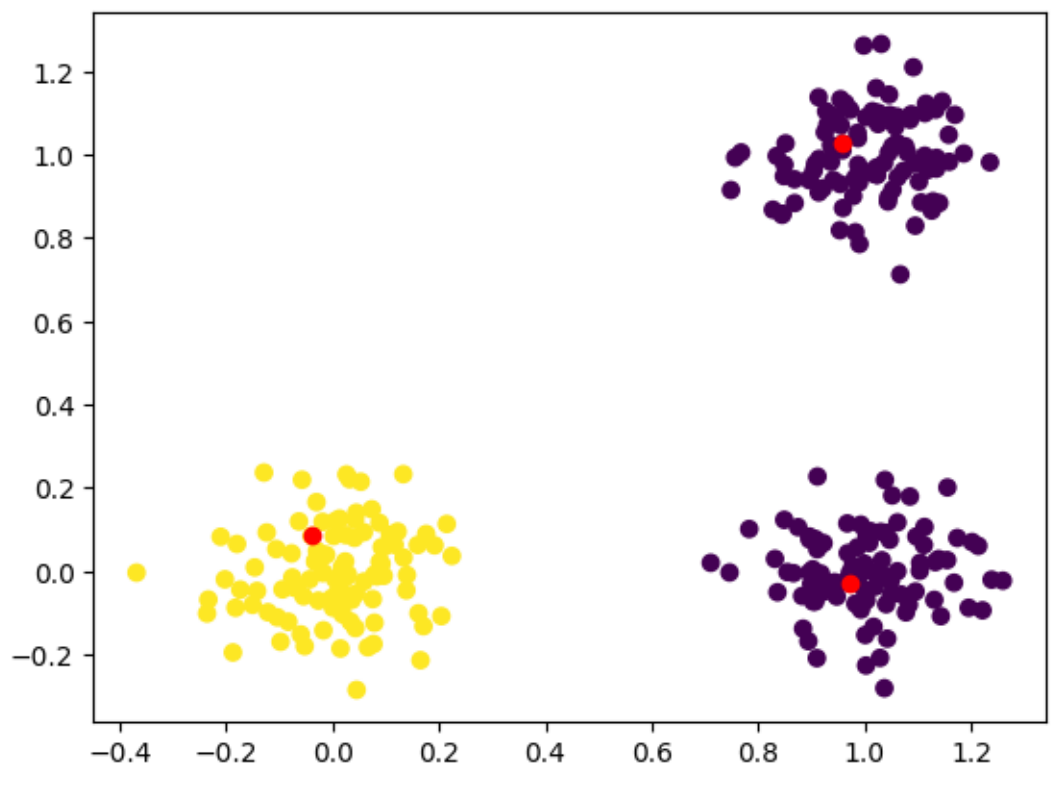
\includegraphics[width=0.8\linewidth]{Figures/Dis3ClusKNNPro.png} 
    \caption{Probit Loss} 
    \label{Fig:Dis3ClusKNNPro} 
  \end{subfigure}%% 
  \begin{subfigure}{0.475\linewidth}
    \centering
    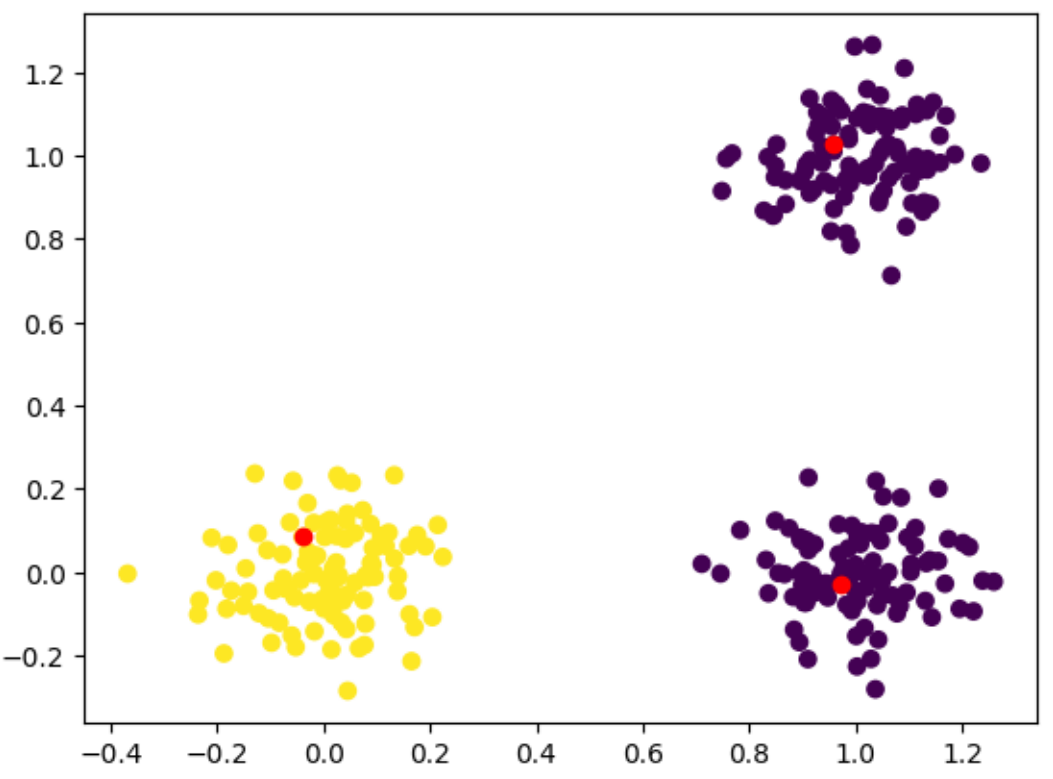
\includegraphics[width=0.8\linewidth]{Figures/Dis3ClusKNNReg.png} 
    \caption{Regression Loss} 
    \label{Fig:Dis3ClusKNNReg} 
  \end{subfigure} 
  \caption{Plot of the predicted labels for the K-NN graph in Figure \ref{Fig:Dis3ClusKNN} and proximity graph in Figure \ref{Fig:Dis3ClusProx}
  using only the known labels.}
  \label{Fig:Dis3ClusKNNRes}
\end{figure}

We repeat the process with the proximity approach. We create a fully connected graph in which the connections between the clusters are of $O(\epsilon)$. Usage of the RBF kernel requires tuning the length scale. We accomplish this by starting with the first quartile of pairwise distances between points and using cross validation on the eigenvalues of $L$ to further tune. We expect three distinct clusters, so there should be a gap between the third and fourth eigenvalues. With the RBF kernel tuned, the proximity graph shown in Figure \ref{Fig:Dis3ClusProx} is produced. Here, it was necessary to tune $\tau$, so that it is $O(\sqrt{\epsilon})$. Doing this resulted in 100\% accuracy for both loss functions and thus produced the same plots as shown in Figure \ref{Fig:Dis3ClusKNNRes}. To ensure that our accuracy results were consistent, we computed the average accuracy over 50 trials of each of the cases. These results are shown in Table \ref{Table:3ClusRes}.

\begin{table}
\begin{center}
\begin{tabular}{||c c c||} 
 \hline
 Type of Graph & Loss Function & Average Accuracy\\  
 \hline\hline
 Disconnected (K-NN) & Probit & 100\% \\ 
 \hline
 Disconnected (K-NN) & Regression & 100\% \\
 \hline
 Weakly Connected (Proximity) & Probit & 100\% \\
 \hline
 Weakly Connected (Proximity) & Regression & 100\% \\ 
 \hline
\end{tabular}
\caption{Average Accuracy of predicted labels over 50 runs for both a fully disconnected and a weakly connected graph using both probit and regression loss functions.}
\label{Table:3ClusRes}
\end{center}
\end{table}

\subsection{Clusters on the Swiss Roll}

Consider the Swiss roll manifold described by $(x,y) = (t\cos(t), t\sin(t))$. We begin by generating points to form well-separated clusters on this manifold. These clusters are formed by specifying a range of $t$-values for which each cluster will be defined, a variance for how far the points will vary from the true manifold, and the number of points to be generated. To avoid majority labelling we ensure that there are the same number of points labeled for each class. A plot of the clusters formed using this process is shown in Figure~\ref{Fig:SpiOg}.
\begin{figure}
    \centering
    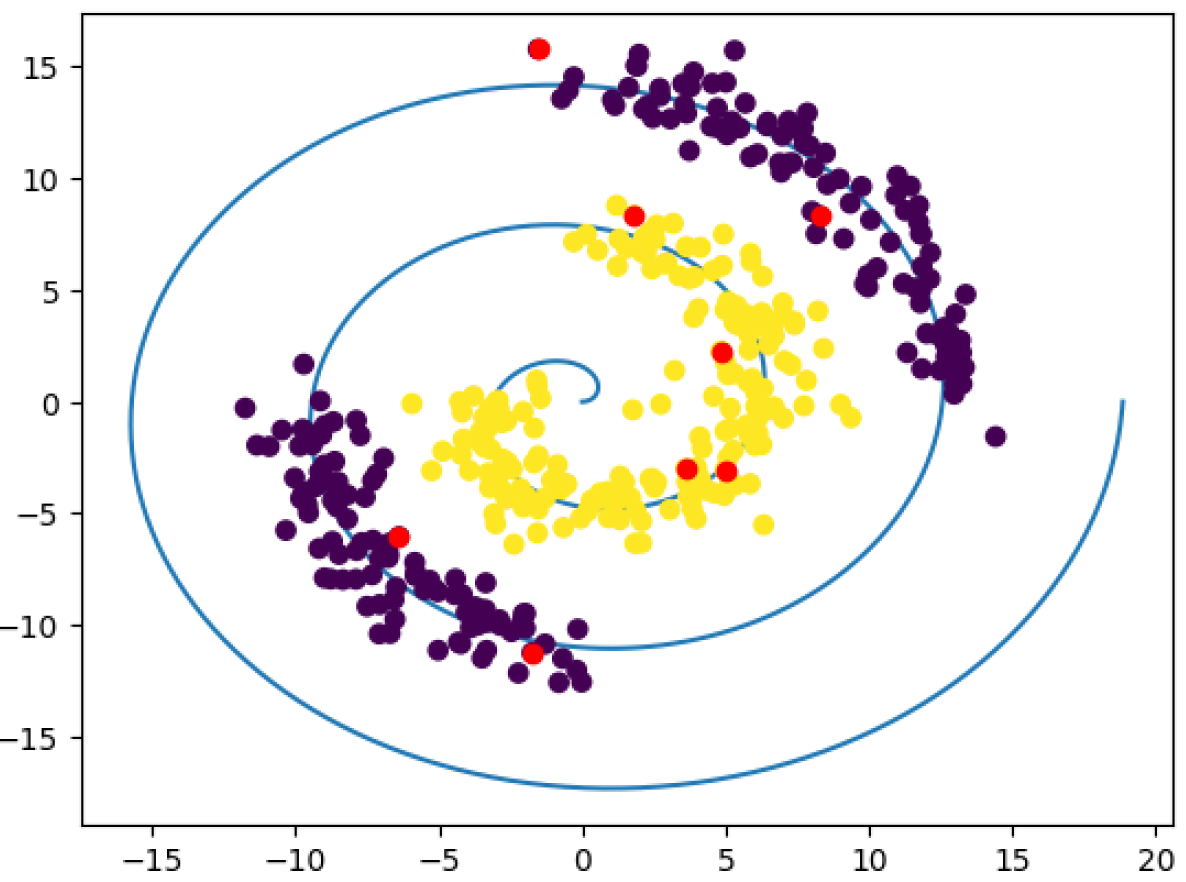
\includegraphics[width=0.5\textwidth]{Figures/SpiOg.png}
    \caption{
        Plot of the 3 clusters on the Swiss roll manifold with $t$-ranges $[\pi,5\pi/2]$, $[3\pi,7\pi/2]$, and $[4\pi,9\pi/2]$ with variance $1$. The blue sprial represents the true swiss roll manifold for which our clusters are generated around.
    }
	\label{Fig:SpiOg}
\end{figure}

We choose to construct three different types of graphs for this example: a K-NN graph with uniform weights, a K-NN graph with the Gaussian weights, and a proximity graph with Gaussian weights. We tune the parameters for all of these approaches using the method described previously. Graphs formed using each of these techniques is shown in Figure \ref{Fig:SpiGraphs}.
    \begin{figure}[ht] 
  \begin{subfigure}{0.475\linewidth}
    \centering
    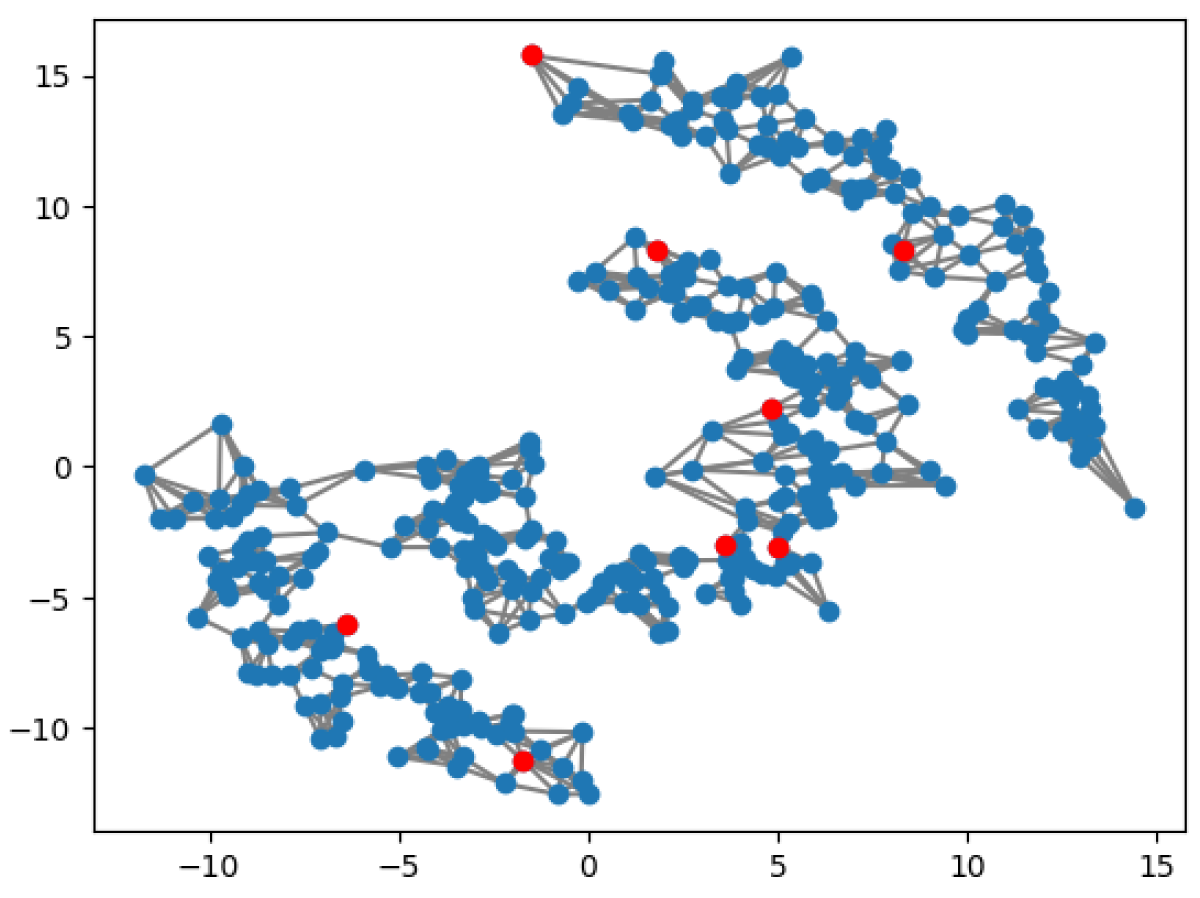
\includegraphics[width=0.8\linewidth]{Figures/SpiKNNUni.png} 
    \caption{K-NN with uniform kernel} 
    \label{Fig:SpiKNNUni}
  \end{subfigure}%% 
  \begin{subfigure}{0.475\linewidth}
    \centering
    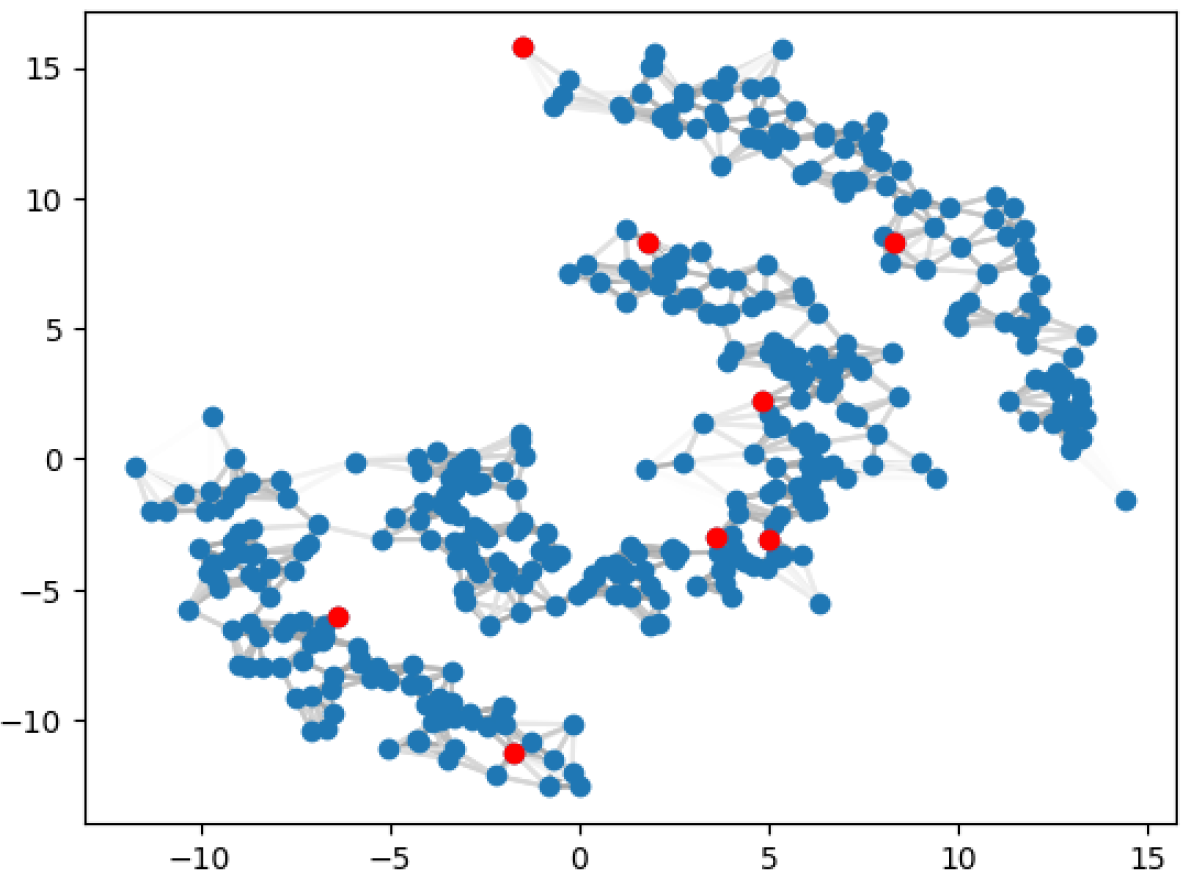
\includegraphics[width=0.8\linewidth]{Figures/SpiKNNRBF.png} 
    \caption{K-NN with RBF kernel} 
    \label{Fig:SpiKNNRBF}
  \end{subfigure} 
    \begin{subfigure}{0.475\linewidth}
    \centering
    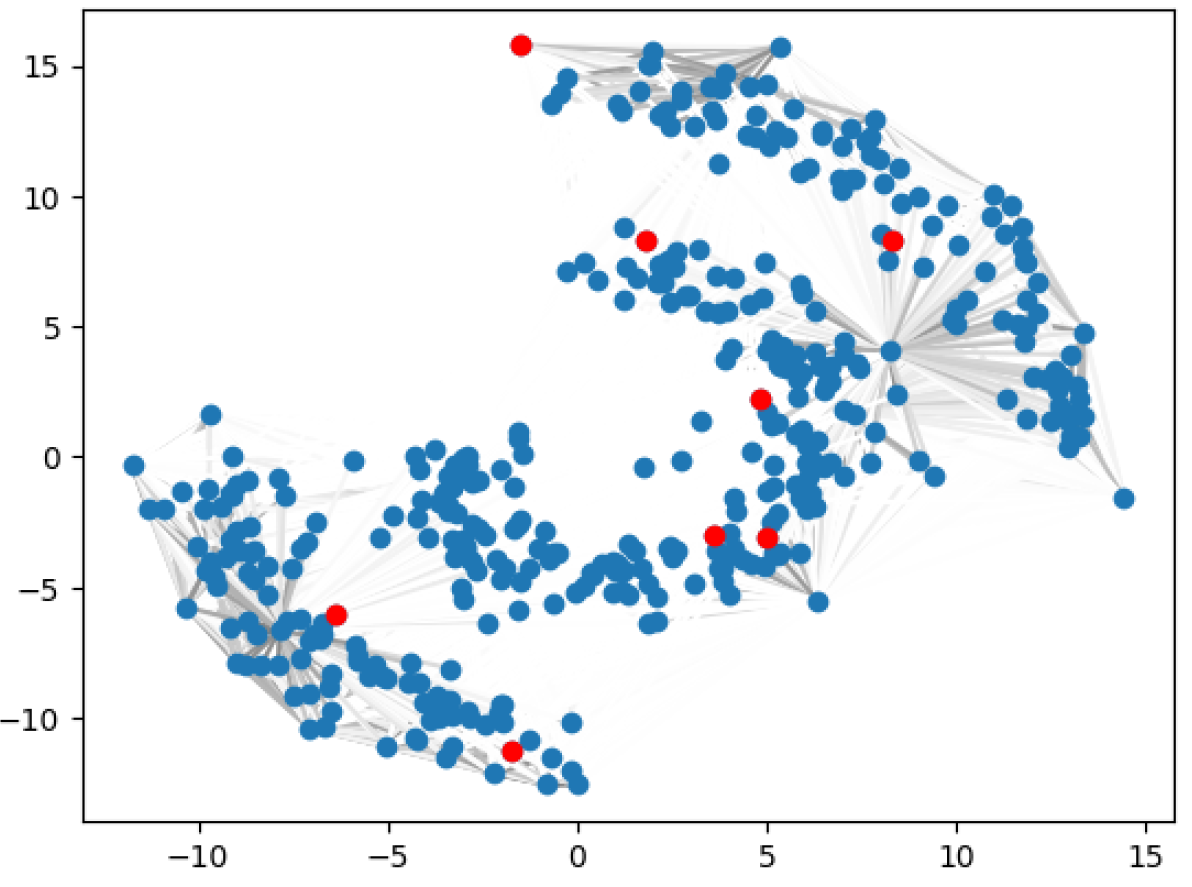
\includegraphics[width=0.8\linewidth]{Figures/SpiProx.png} 
    \caption{Proximity with RBF kernel} 
    \label{Fig:SpiProx}
  \end{subfigure} 
  \caption{Plot of the graphs formed for the data in Figure~\ref{Fig:SpiOg}. Each subfigure shows a different graph forming technique.}
  \label{Fig:SpiGraphs} 
\end{figure}
We then perform our GSSL algorithm with both the Probit loss and regression loss. Plots of the predicted labels using both the Probit and regression loss functions for each type of graph are shown in Figure \ref{Fig:SpiPred}.
    \begin{figure}[ht] 
  \begin{subfigure}{0.475\linewidth}
    \centering
    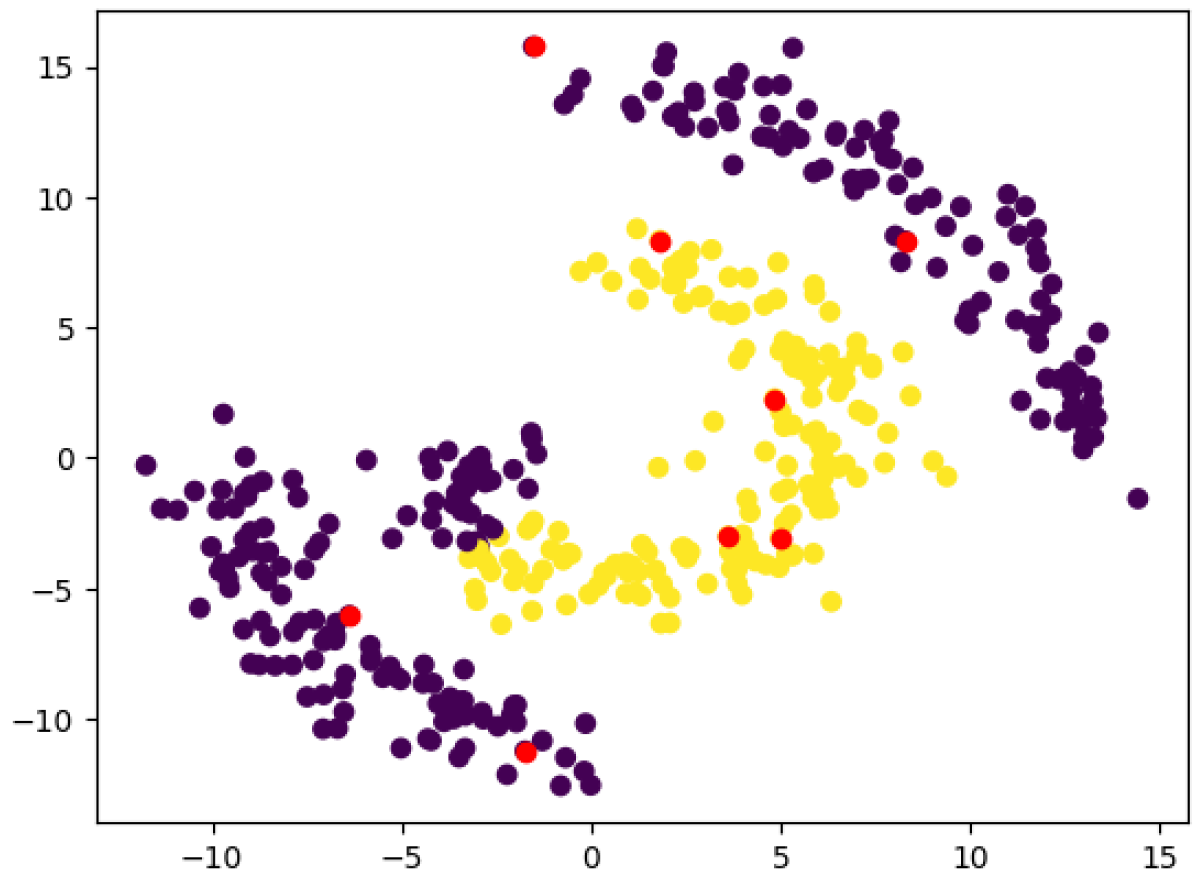
\includegraphics[width=0.8\linewidth]{Figures/SpiKNNUniPro.png} 
    \caption{K-NN with uniform weights: Probit} 
    \label{Fig:SpiKNNUniPro} 
  \end{subfigure}%% 
  \begin{subfigure}{0.475\linewidth}
    \centering
    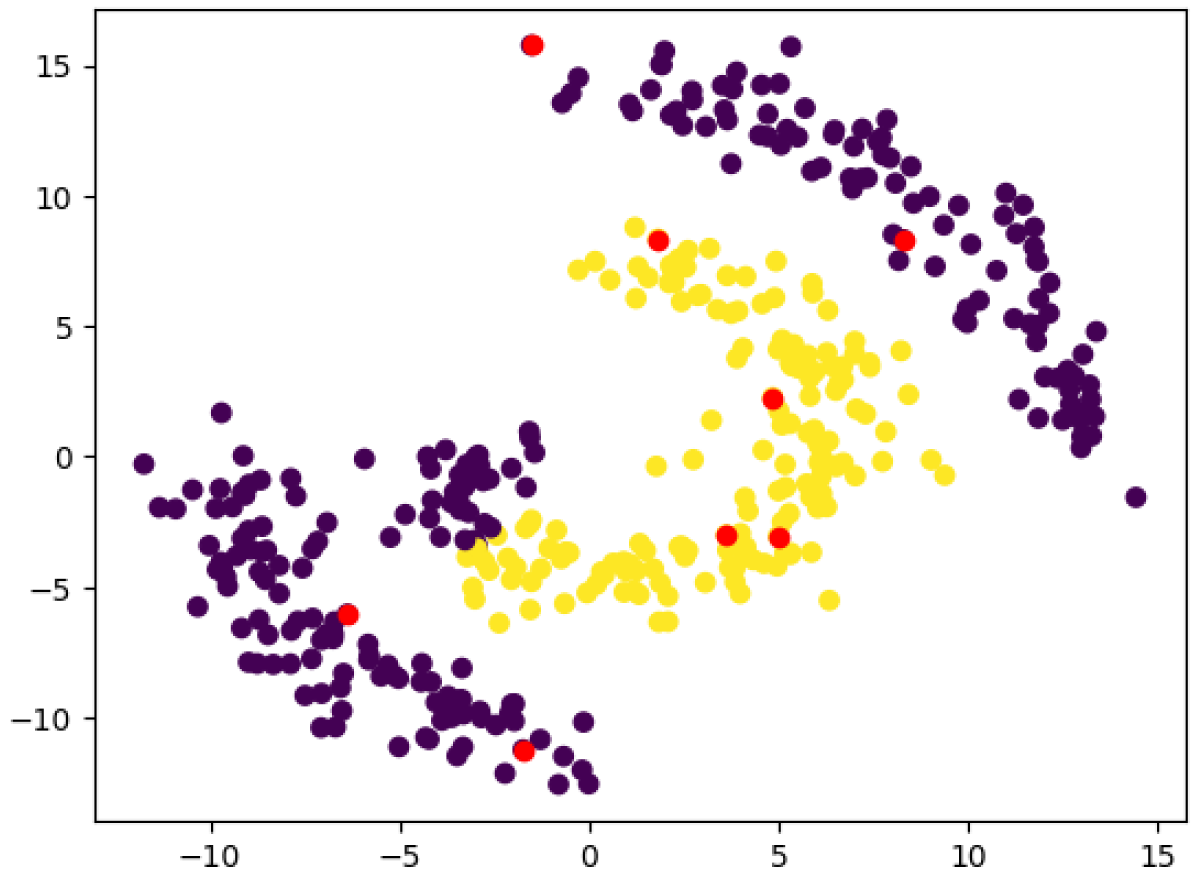
\includegraphics[width=0.8\linewidth]{Figures/SpiKNNUniReg.png} 
    \caption{K-NN with uniform weights: Regression} 
    \label{Fig:SpiKNNUniReg} 
  \end{subfigure} 
    \begin{subfigure}{0.475\linewidth}
    \centering
    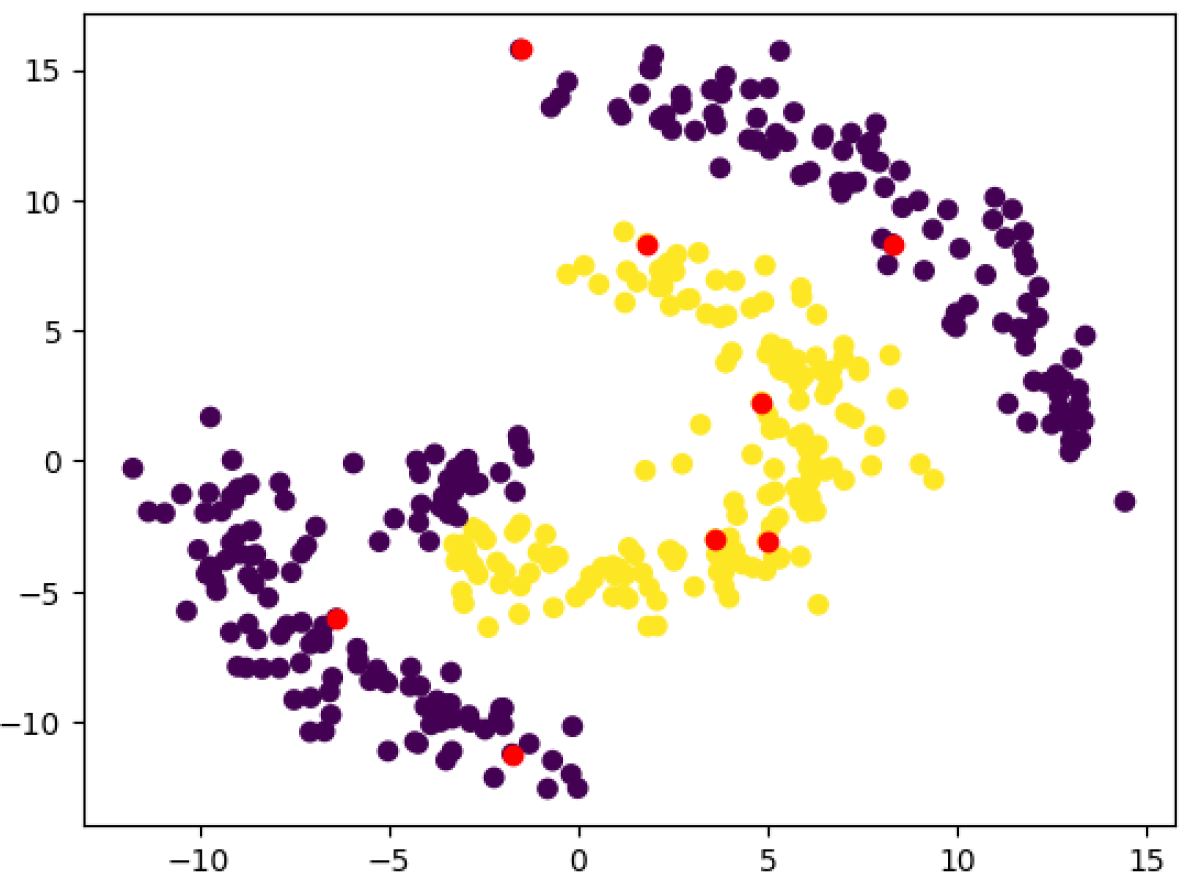
\includegraphics[width=0.8\linewidth]{Figures/SpiKNNRBFPro.png} 
    \caption{K-NN with Gaussian weights: Probit} 
    \label{Fig:SpiKNNRBFPro} 
  \end{subfigure} 
      \begin{subfigure}{0.475\linewidth}
    \centering
    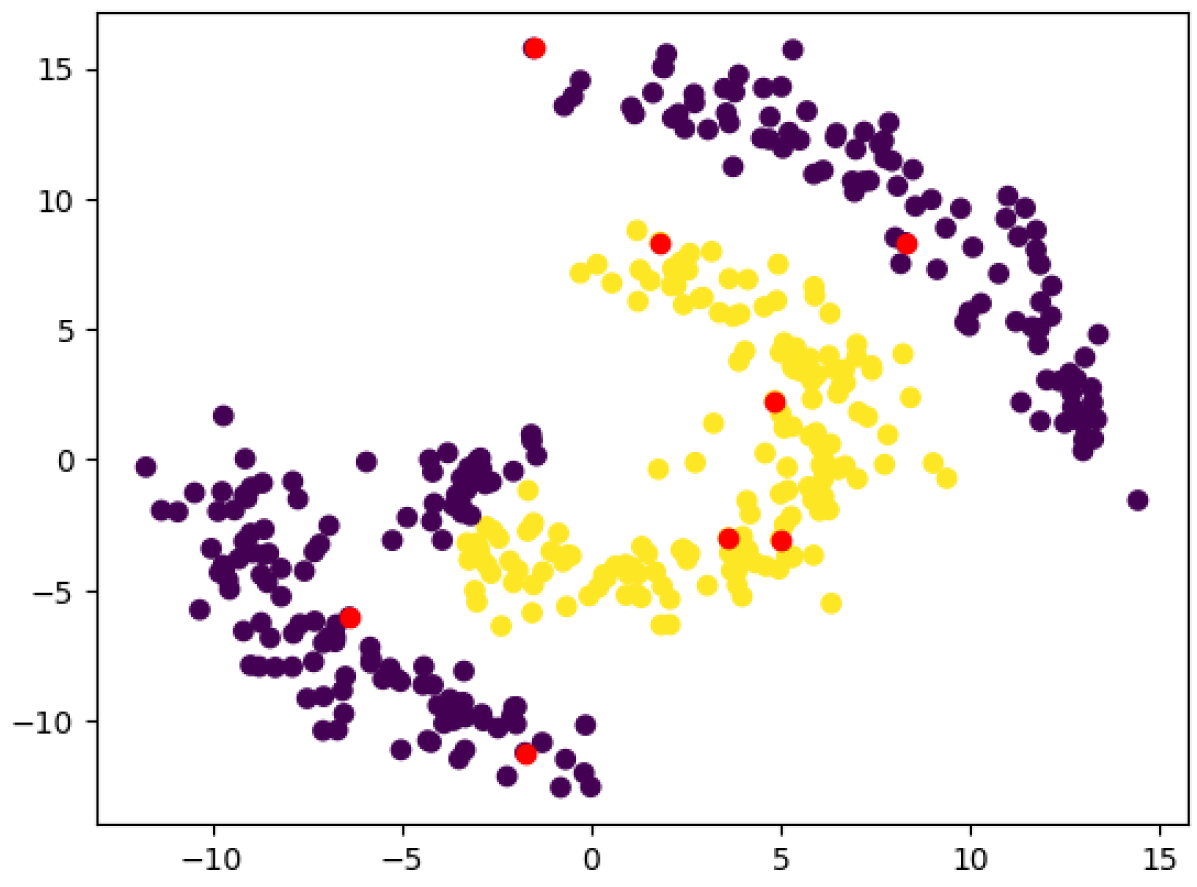
\includegraphics[width=0.8\linewidth]{Figures/SpiKNNRBFReg.png} 
    \caption{K-NN with Gaussian weights: Regression} 
    \label{Fig:SpiKNNRBFReg} 
  \end{subfigure}
      \begin{subfigure}{0.475\linewidth}
    \centering
    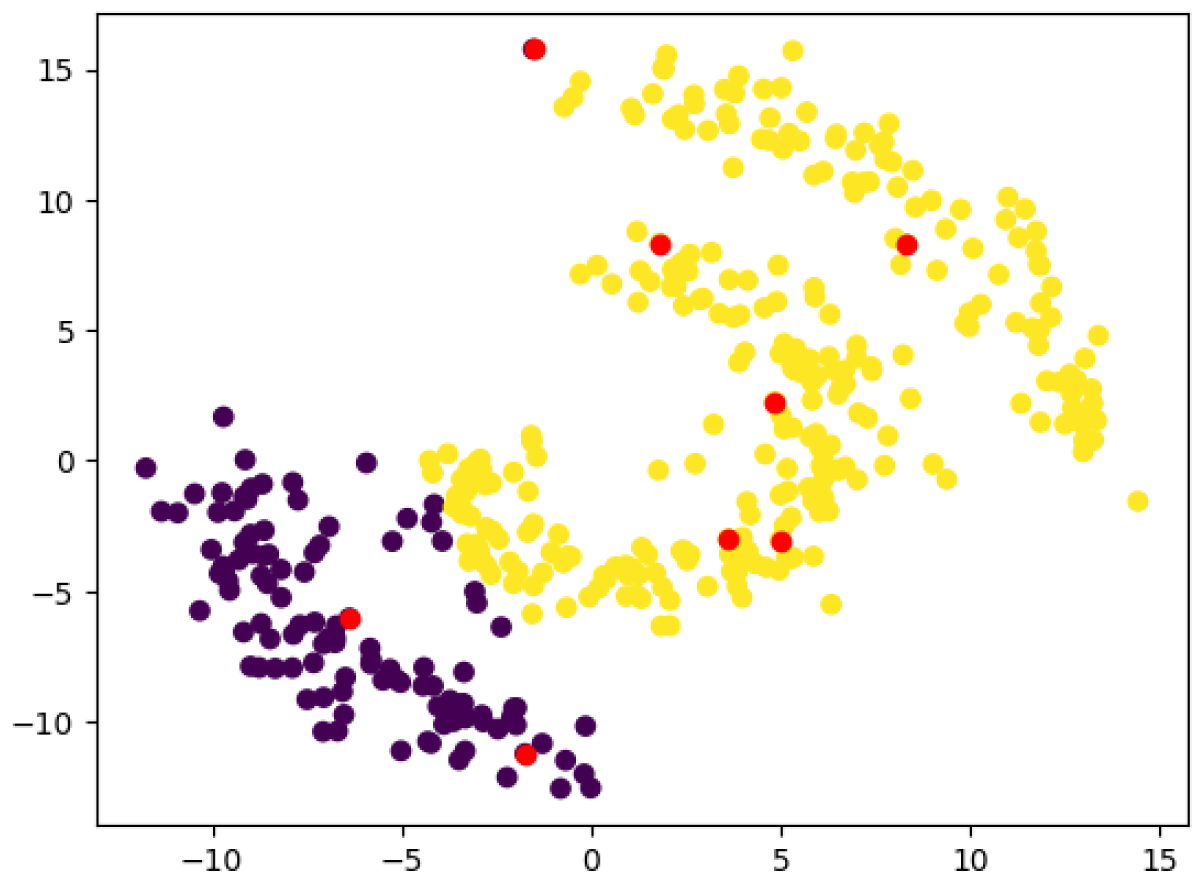
\includegraphics[width=0.8\linewidth]{Figures/SpiProxPro.png} 
    \caption{Proximity with Gaussian weights: Probit} 
    \label{Fig:SpiProxPro} 
  \end{subfigure}
      \begin{subfigure}{0.475\linewidth}
    \centering
    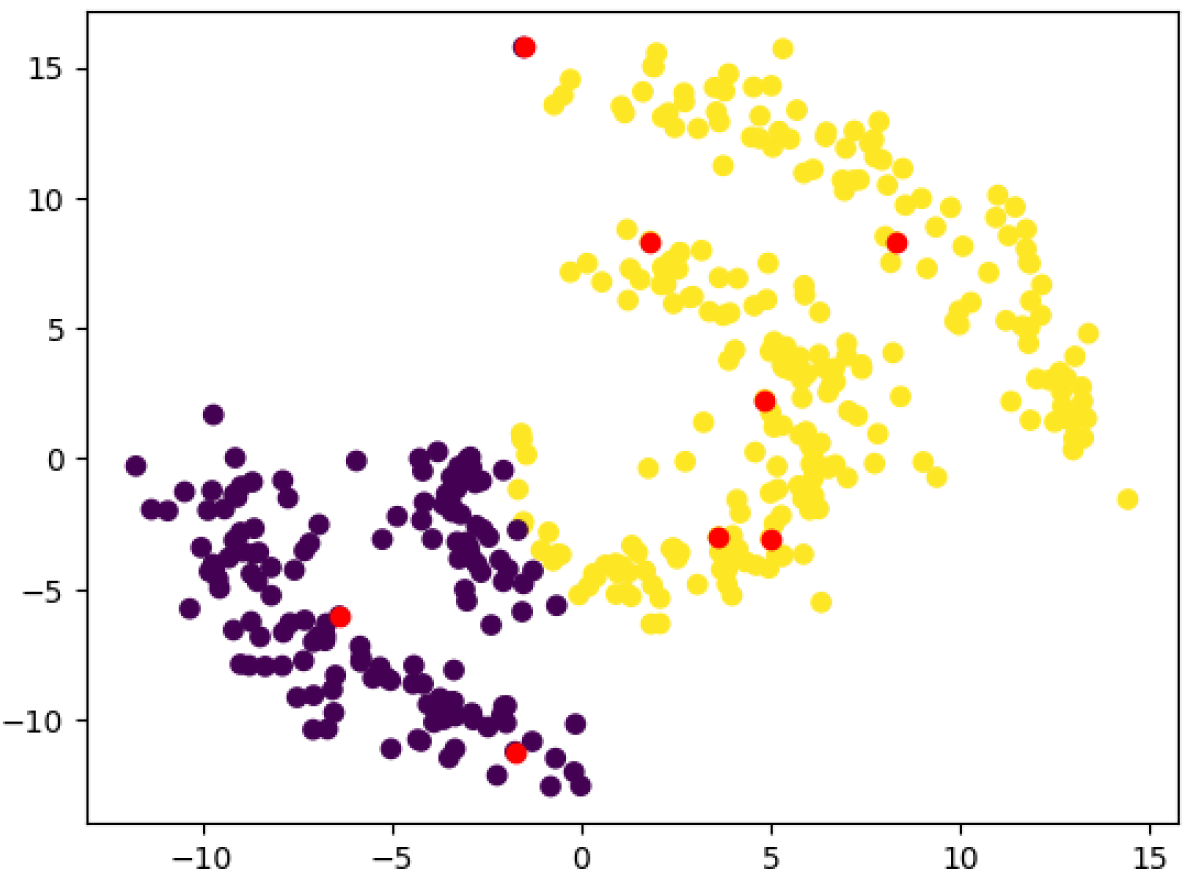
\includegraphics[width=0.8\linewidth]{Figures/SpiProxReg.png} 
    \caption{Proximity with Gaussian weights: Regression} 
    \label{Fig:SpiProxReg} 
  \end{subfigure}
  \caption{Plot of the predicted labels for the clusters generated on the Swiss roll manifold using the graphs generated in Figure \ref{Fig:SpiGraphs}. }
  \label{Fig:SpiPred} 
\end{figure}
The accuracies of the predicted labels compared to the true labels for each type of graph and each loss function are shown in Table \ref{Table:SpiRes}.

\begin{table}
\begin{center}
\begin{tabular}{||c c c c||} 
 \hline
 Type of Graph & Loss Function & 1 Trial Accuracy & 50 Trial Avg. Accuracy\\ 
 \hline\hline
 K-NN with uniform kernel & Probit & 91.00\% & 94.80\%\\ 
 \hline
 K-NN with uniform kernel & Regression & 91.00\% & 93.51\%\\
 \hline
 K-NN with RBF kernel & Probit & 92.25\% & 96.30\%\\
 \hline
 K-NN with RBF kernel & Regression & 92.50\% & 95.76\%\\
 \hline
 Proximity with RBF kernel & Probit & 73.00\% & N/A\\
 \hline
 Proximity with RBF kernel & Regression & 63.00\% & N/A\\
 \hline
\end{tabular}
\caption{Accuracy of predicted labels over 1 run and average accuracy over 50 runs for 3 different types of graphs using both probit and regression loss functions. Note that we did not perform 50 trials for the proximity graph with the Gaussian weights as this approach performed poorly in our initial tests.}
\label{Table:SpiRes}
\end{center}
\end{table}
We can see from Figure \ref{Fig:SpiPred} and Table \ref{Table:SpiRes} that the proximity graph with the RBF kernel performs poorly in comparison with both of the K-NN graphs that both have over $90\%$ accuracy. Thus, we proceed only with the two K-NN graphs. To ensure the consistency of the success of the K-NN kernels, we computed the average accuracy over 50 trials for the two K-NN graphs with both the probit and regression loss functions. The average accuracy of over these 50 trials are shown in Table \ref{Table:SpiRes}. 

\subsection{MNIST Data}
We now consider applying our GSSL algorithm to real data. In this case, we consider a subset of the MNIST data set. In particular, we look at 500 randomly chosen images from the complete set of 0s and 1s. We assigned each 0 a true label of -1 and each 1 a true label of 1. Thirty points in the data set are then assigned their true label. We next construct a K-NN graph with Gaussian weights. We then perform our GSSL algorithm with both the Probit and regression loss functions. After cross-validation, we found that the ideal parameters were given by: $\gamma=0.04$, $\tau=1$, $\alpha=2$, and $\lambda=\tau^{2\alpha}/2$. These parameters resulted in the formation of two clusters, as desired. Our approach predicted labels with $89.6\%$ accuracy for the Probit loss function and $90.8\%$ accuracy for the regression loss function, showing that our approach is effective on real data.

\section{Conclusions}
Graphical semi-supervised learning is a useful tool that combines the strengths of both supervised and unsupervised learning methods. Using information from both labeled and unlabeled data allows for the development of robust machine learning models that require less information than traditional approaches. However, this approach is not without its limitations. The quality of the graph construction, the choice of kernel, and the selection of labeled points all have an impact on the final performance of the model.

\nocite{hoffmann, borovitskiy, sanz-alonso}
\bibliographystyle{plain}
\bibliography{bibliography_file}

\section{Appendix}
The code for this project can be found here:

https://github.com/rohingilman/AMATH563\_gssl
\end{document}